\documentclass[a4paper, 12pt]{book}

\usepackage[T1]{fontenc}
\usepackage[utf8]{inputenc}
\usepackage[italian]{babel}
\usepackage{quoting}
\usepackage{graphicx} %per inserire immagini nel testo
\usepackage{sidecap} %permette di aggiungere didascalie alle immagini
\usepackage{subfig}
\usepackage[colorlinks]{hyperref} %per rendere interattivo il documento, gli elementi interattivi saranno in rosso con l'opzione colorlinks
\usepackage{amsmath}
\usepackage{amsthm} %per enunciati
\theoremstyle{plain}
\newtheorem{teorema}{Teorema}[section]
\usepackage{geometry}
\geometry{a4paper, top = 3cm, bottom = 3cm, left = 3.5cm, right = 3.5cm, heightrounded, bindingoffset = 5mm}
\pagestyle{plain}
\usepackage{multirow}

\title{Titolo \\ riga sotto}
\author{Autore \thanks{Ringraziamenti}}
\date{giorno mese anno}  

\setcounter{secnumdepth}{3}
%\setcounter{tocdepth}{1}

\begin{document}
	\begin{titlepage}
		\maketitle
	\end{titlepage}

	\frontmatter %numeri romani prima del testo effettivo
	\tableofcontents
	\mainmatter %numeri arabi dalla prima pagina di testo effettivo

	\chapter{Cose utili}
	
	\section{Sezione numerata}
	
	\section*{Sezione non numerata}
	
	\section{Capoversi}
	
	\subsection{Metodo 1}
	
	Un capoverso si può formare mettendo una riga vuota tra una riga e l'altra. Per esempio la prossima riga sarà un nuovo capoverso.
	
	Ecco il nuovo capoverso con il metodo sopracitato.
	
	\subsection{Metodo 2}
	
	 Un secondo metodo per inserire un nuovo capoverso è attraverso il comando \textbf{$\backslash$par}. \par Ecco un nuovo capoverso.
	
	\section{Note}
	
	\subsection{A margine}
	
	Tramite il comando \textbf{$\backslash$marginpar} è possibile creare una nota\marginpar{Questa è una nota al margine} al margine del foglio.
	
	\subsection{A piè di pagina}
	
	Tramite il comando \textbf{$\backslash$footnote} si creano note\footnote{Questa è una nota a piè di pagina} in fondo al foglio. Ogni volta le note vengono numerate così da poterle distinguere\footnote{Questa è una seconda nota}.
	
	\section{Ambienti testuali}
	\subsection{Elenchi}
	Elenco puntato:
	\begin{itemize}
		\item Primo punto.
		\item Secondo punto.
		\begin{itemize}
			\item Sotto elenco puntato.
			\item Secondo sotto punto.
			\begin{itemize}
				\item Terzo livello di elenco puntato.
				\begin{itemize}
					\item Quarto livello di elenco puntato.
					\item [+] Punto personalizzato.
					\item [>] Punto personalizzato.
				\end{itemize}
			\end{itemize}
		\end{itemize}
	\item [@] Terzo punto.
	\end{itemize}

	\begin{enumerate}
		\item Primo punto.
		\item Secondo punto.
		\begin{enumerate}
			\item Sotto elenco numerato.
			\item Secondo sotto punto.
			\begin{enumerate}
				\item Terzo livello di elenco numerato.
				\begin{enumerate}
					\item Quarto livello di elenco numerato.
					\item Nuovo elemento.
				\end{enumerate}
			\item Altro elemento.
			\end{enumerate}
		\end{enumerate}
	\end{enumerate}
	
	\section{Citazioni}
	
	Per inserire una citazione serve il pacchetto \textbf{quoting}, successivamente le si inserisce tramite il comando \textbf{$\backslash$begin{quoting}}.
	
	\begin{quoting}
		La citazione verrà scritta al centro.
	\end{quoting}

	\section{Formule matematiche}
	\subsection{Tipologie di formule}
	\subsubsection{Formula inline}
	Esistono tre modi per generare le \textbf{formula inline}:
	\begin{enumerate}
		\item Doppio uso del dollaro: $10\cdot 5 = 50$.
		\item Parentesi tonde precedute dal backslash \(45 / 3 = 15\).
		\item Ambiente matematico \textbf{math}: \begin{math}
		37 - 14 = 23
		\end{math}
	\end{enumerate}
	\LaTeX cerca di comprimere il meglio possibile $\sum_{x=1}^{10}\frac{x}{5} = 11$ le formule matematiche in linea.
	
	\subsubsection{Formula in display}
	Esistono tre modi per generare la \textbf{formula in display}:
	\begin{enumerate}
		\item Ambiente matematico \textbf{equation}
		\begin{equation}
		v = \frac{s}{t}
		\end{equation}
		\item Parentesi quadre precededute dal backslash $\backslash$[
		\[
		rad = \frac{\pi}{180}\theta
		\]
		\item Ambiente matematico \textbf{displaymath}:
		\begin{displaymath}
		\alpha = \frac{\Delta\omega}{\Delta t}
		\end{displaymath}
	\end{enumerate}

	\subsection{Opzioni interessanti}
	\subsubsection{Affiancare più espressioni}
	Per affiancare più espressioni all'interno di un singolo ambiente si fa uso dei comandi: \textbf{$\backslash$quad} e \textbf{$\backslash$qquad} per spaziare le due formule.
	\[
	y = mx + q\qquad y = \frac{x - q}{m}
	\]
	\subsubsection{Inserire una piccola porzione di testo}
	Per inserire una piccola porzione di testo all'interno dell'ambiente si utilizza \textbf{$\backslash$textrm}:
	\[
	y = \sqrt{x} \quad\textrm{per $x\geq 0$}
	\]
	
	\subsubsection{Inserzioni}
	Si possono scrivere delle annotazioni sopra o sotto alle espressioni tramite il comando \textbf{$\backslash$underbrace} o \textbf{$\backslash$overbrace}:
	\[
	\underbrace{1 + 2, \dots, n}_{\frac{n(n + 1)}{2}} + (n + 1)\qquad \overbrace{1 + 2, \dots, n}^{\frac{n(n + 1)}{2}} + (n + 1)
	\]
	
	\subsubsection{Sistemi di equazioni}
	Per creare sistemi di equazioni si usa l'ambiente matematico \textbf{case}:
	\[
	\begin{cases}
		x + y = 2\\
		x - y = 0
	\end{cases}
	\]
	
	\subsubsection{Vettori e matrici}
	\begin{itemize}
		\item Matrice e vettori senza parentesi:
		\[
		\begin{matrix}
			1 & 1 & \dots & 1\\
			\vdots & \vdots & \ddots & \vdots\\
			1 & 1 & \dots & 1
		\end{matrix} \qquad \begin{matrix}
			1 & 1 & \dots & 1
		\end{matrix} \qquad \begin{matrix}
			1\\
			\vdots\\
			1
		\end{matrix}
		\]
		\item Matrice e vettori con parentesi tonde:
		\[
		\begin{pmatrix}
			1 & 1 & \dots & 1\\
			\vdots & \vdots & \ddots & \vdots\\
			1 & 1 & \dots & 1
		\end{pmatrix} \qquad \begin{pmatrix}
			1 & 1 & \dots & 1
		\end{pmatrix} \qquad \begin{pmatrix}
			1\\
			\vdots\\
			1
		\end{pmatrix}
		\]
		\item Matrice e vettori con linea:
		\[
		\begin{vmatrix}
			1 & 1 & \dots & 1\\
			\vdots & \vdots & \ddots & \vdots\\
			1 & 1 & \dots & 1
		\end{vmatrix} \qquad \begin{vmatrix}
			1 & 1 & \dots & 1
		\end{vmatrix} \qquad \begin{vmatrix}
			1\\
			\vdots\\
			1
		\end{vmatrix}
		\]
		\item Matrice e vettori con doppia linea:
		\[
		\begin{Vmatrix}
			1 & 1 & \dots & 1\\
			\vdots & \vdots & \ddots & \vdots\\
			1 & 1 & \dots & 1
		\end{Vmatrix} \qquad \begin{Vmatrix}
			1 & 1 & \dots & 1
		\end{Vmatrix} \qquad \begin{Vmatrix}
			1\\
			\vdots\\
			1
		\end{Vmatrix}
		\]
	\end{itemize}

	\subsubsection{Raggruppamento e gestione delle formule}
	Per spezzare una formula lunga si utilizza \textbf{multiline}:
	\begin{multline}
		z = a + b + c + d\\
		+ e + f + g + h\\
		+ i + l + m + n\\
		+ o + p + q + r\\
		+ s + t + u + v
	\end{multline}
	Per incolonnarla invece si utilizza \textbf{split}:
	\[
	\begin{split}
		z &= a + b + c + d\\
		&= e + f + g + h\\
		&= i + l + m + n\\
		&= o + p + q + r\\
		&= s + t + u + v
	\end{split}
	\]
	Per raggrupparle si utilizza \textbf{gather}:
	\begin{gather}
		y = mx + q\\
		y = ax^2 + bx + c\\
		y = \sin(x)
	\end{gather}
	Per raggrupparle incolonnate si utilizza \textbf{align}:
	\begin{align}
		y &= mx + q & y &= ax^2 + bx + c & y &= \sin(x)\\
		x^2 + y^2 + ax + by + c &= 0 & xy &= k & y &= \tan(x)
	\end{align}
	
	\subsubsection{Teoremi}
	Sono tre opzioni:
	\begin{itemize}
		\item \textbf{plain}
		\item \textbf{definition}
		\item \textbf{remark}
	\end{itemize}
	Si deve specificare lo stile all'inizio con \textbf{$\backslash$theoremstyle{}}
	inserendo all'interno delle parentesi graffe l'eventuale stile scelto.
	Successivamente per enunciare un nuovo teorema si scriverà
	\textbf{$\backslash$newtheorem{teorema}{Teorema}[section]}
	\begin{teorema}[Nome teorema]
		Bla bla bla bla.
	\end{teorema}	
	L'eventuale dimostrazione si fa usando \textbf{$\backslash$proof}:
	\begin{proof}
		Cose varie bla bla bla.
	\end{proof}	
	Notare la presenza di una quadratino alla fine per indicare che la 
	dimostrazione è stata completata.

	\section{Importare immagini}
	Le immagini vengono importate aggiungendo il pacchetto
	\textbf{graphicx} e utilizzando il comando \textbf{$\backslash$includegraphicx[opzioni]\{nome immagine\}}:\\
	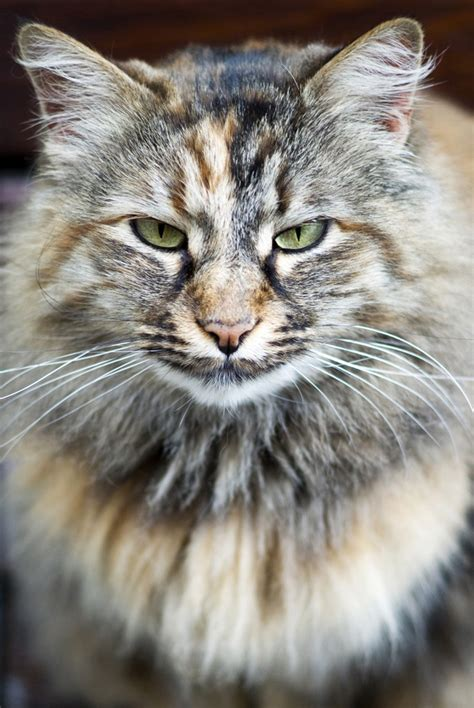
\includegraphics[width=0.3\textwidth]{cat.jpeg}

	\subsection{Didascalie laterali}
	Tramite il comando \textbf{$\backslash$SCfigure[opzioni][opzioni]}:
	\begin{SCfigure}[50][h!]
		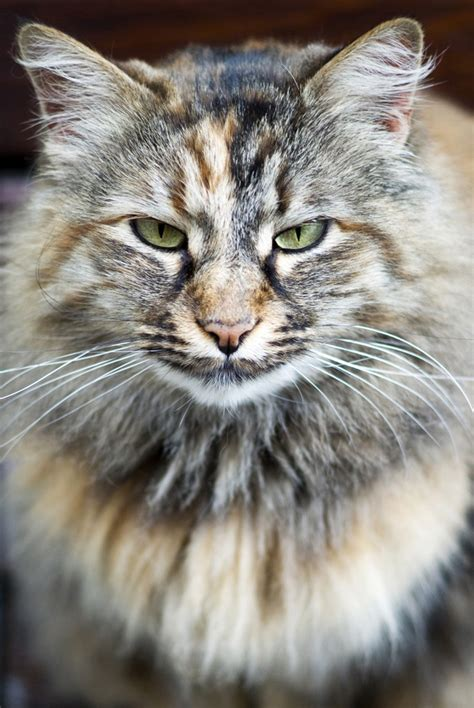
\includegraphics[width=0.3\textwidth]{cat.jpeg}
		\caption{Questo è un gatto norvegese}
	\end{SCfigure}
	\subsubsection{Multiple immagini}
	Con l'ambiente \textbf{figure[opzioni]} è possibile
	inserire più immagini assieme. 
	\begin{figure}[h!]
		\centering
		\subfloat[][\textbf{\emph{Questo gatto è bellissimo}}]
		{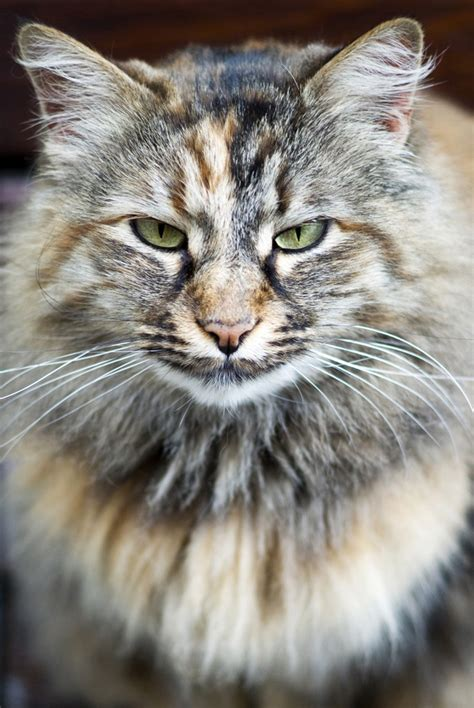
\includegraphics[width=0.3\textwidth]{cat.jpeg}}\quad
		\subfloat[][\textbf{\emph{Anche questo gatto è bellissimo}}]
		{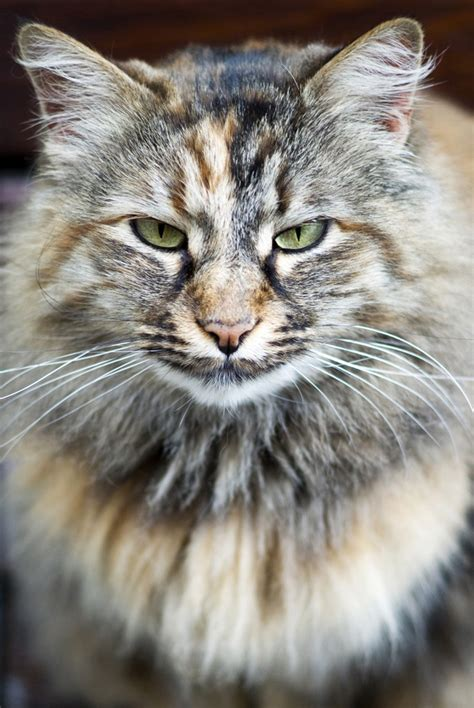
\includegraphics[width=0.3\textwidth]{cat.jpeg}}\\
		\subfloat[][\textbf{\emph{Questo cane è bellissimo}}]
		{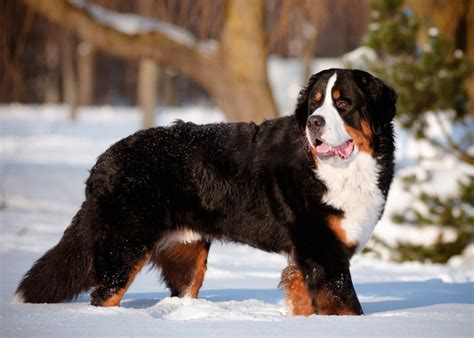
\includegraphics[width=0.3\textwidth]{dog.jpeg}}\quad
		\subfloat[][\textbf{\emph{Anche questo cane è bellissimo}}]
		{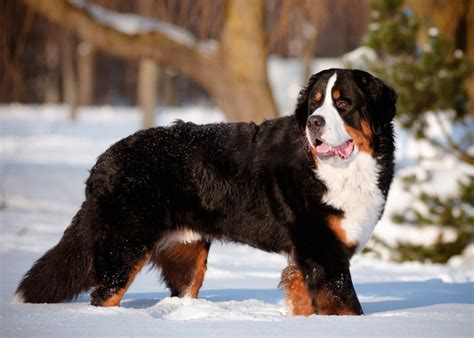
\includegraphics[width=0.3\textwidth]{dog.jpeg}}
		\caption{Dentro all'ambiente \textbf{$\backslash$figure} ci sono quattro
		sotto figure}
	\end{figure}

	\section{Creare tabelle}
	L'ambiente predisposto per le tabelle è \textbf{tabular}, 
	dove all'interno delle graffe si specificano i descrittori delle colonne:
	\begin{center}
		\begin{tabular}{l c r}
			Cella 1 & Cella 2 & Cella 3\\
			Cella 4 & Cella 5 & Cella 6\\
			Cella 7 & Cella 8 & Cella 9\\
		\end{tabular}
	\end{center}
	Le opzioni fornite sono:
	\begin{description}
		\item[l] allinea il contenuto della cella a sinistra
		\item[c] centra il contenuto della cella
		\item[r] alline il contenuto della cella a destra
		\item[p] giustifica un testo lungo entro una larghezza
		\item[*] ripete i descrittori  
	\end{description}
	Per ottenere delle linee verticali si inserisce \textbf{|} tra 
	un'opzione e l'altra:
	\begin{center}
		\begin{tabular}{l | c | r}
			Cella 1 & Cella 2 & Cella 3\\
			Cella 4 & Cella 5 & Cella 6\\
			Cella 7 & Cella 8 & Cella 9\\
		\end{tabular}
	\end{center}
	Per inserire quelle orizzontali si usa \textbf{$\backslash$hline}:
	\begin{center}
		\begin{tabular}{l c r}
			\hline
			Cella 1 & Cella 2 & Cella 3\\
			\hline
			Cella 4 & Cella 5 & Cella 6\\
			\hline
			Cella 7 & Cella 8 & Cella 9\\
			\hline
		\end{tabular}
	\end{center}
	Per unire più colonne si usa il comando \textbf{$\backslash$multicolumn{n elementi}{eventuali righe}{Nome}}:
	\begin{center}
		\begin{tabular}{| c | c | c |}
			\hline
			\multicolumn{3}{| c |}{Unione}\\
			\hline
			Cella 4 & Cella 5 & Cella 6\\
			\hline
			Cella 7 & Cella 8 & Cella 9\\
			\hline
		\end{tabular}
	\end{center}
	Stessa cosa per le righe, \textbf{$\backslash$multirow}:
	\begin{center}
		\begin{tabular}{| c | c | c |}
			\hline
			\multirow{3}{4em}{Unione} & Cella 2 & Cella 3\\
			& Cella 5 & Cella 6\\
			& Cella 8 & Cella 9\\
			\hline
		\end{tabular}
	\end{center} 
	
	
	
\end{document}
